\section{New MBSA Capabilities}

\mike{REWRITE!}

Previous research has been based on MBD tools (such as Simulink and SCADE) that were available at the time \cite{Joshi05:Dasc}. However, these tools are really targeted at the design and implementation of software components, rather than at the system architecture level where most safety concerns arise.

Within the past five years there have been great advances in the capabilities of tools for modeling and analysis of at the system level, based on languages such as SysML \cite{SysML} and AADL \cite{AADL}. We use these new MBSE capabilities and extend them to implement the safety analysis methods needed for the design and certification of commercial aircraft systems. The system modeling tools that we plan to use are based on AADL, but they can import and export models from SysML.

\begin{itemize}
\item We will improve the efficiency of MBSA methods by using MBSE tools that can perform compositional reasoning over complex system models. Using the assume- guarantee contract mechanism, these tools provide support for heterogeneous component models implemented in different languages (such as Simulink or C/C++).

\item Our new analysis methods move away from traditional static safety analysis methods focused on probabilistic models (e.g., Fault Tree Analysis), to the direct modeling of potential failure mechanisms and the analysis of dynamic fault-mitigation strategies.

\item Formal verification of system models provides increased assurance that these models are accurate and will produce correct results. The hierarchical structure of system architecture models supports analysis at varying levels of abstraction. Compositional analysis explicitly checks assumptions captured in component and subsystem contracts. Consistency and realizability checks [23] provide the ability to detect conflicting requirements between component and subsystem models.
\end{itemize}

%In this section we describe some of the new capabilities that we will develop, including improvements related to the AADL Error Model Annex, the use of model-based assurance cases, and evaluation of system-level certification objectives related to system safety that can be satisfied using the proposed methods.

We bridge the descriptions of errors in the error model annex with behavioral descriptions of components. We start from the error model notions of error types and state machines that describe transitions from nominal to error states. However, we then tie these nominal and error states to behavioral models of the components in question that describe how the faults manifest themselves in terms of the signals or quantities produced by the components. Now the behavioral models can provide implicit propagation of the faulty behaviors and the natural consequences of failures on component behavior will be manifested in the propagation of other component faults through the behavioral model.

To accomplish this, we use AADL and the error model annex to describe faults, and to use the AGREE contract specification language to describe behavioral models. This requires extensions to AGREE to define fault models that describe how different faults manifest themselves in changes to output signals. It also requires changes to the error annex. The conditions under which faults occur will become richer such that they describe not just propagation of enumerations from other components, but also valuations of input signals.

An example is shown in Figure~\ref{fig:error_annex}. Errors are described by the red rectangles labeled with error types: 1-BadData, 2-NoData, 3-NoSvc. Error events that can cause a component to fail are labeled with the corresponding error number. The error behavior of components is described by their state machines. Note that while all state machines in Figure~\ref{fig:error_annex} have two states, they can be much more complex. The red dashed arrows indicate propagations describing how failures in one component can cause other components to fail. For example, failures in the physical layer propagate to failures in the associated logical components.

\begin{figure}
  \centering
 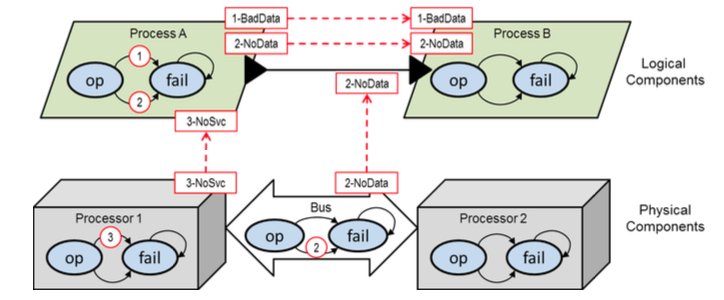
\includegraphics[width=0.75\textwidth]{images/error_annex.png}
  \vspace{-0.1in}
  \caption{Example of Error Model Information and Propagation}
  \label{fig:error_annex}
\end{figure}


%\subsection{Fault and Behavioral Modeling}

